\newpage
\section{Introduction}

Cavity electrodynamics is the study of light confined inside an optical resonater and hence quantized as a basis of harmonic oscillator modes. The quantization of the electromagnetic (EM) field inside an optical cavity has been, and continues to be, paramount in the advancement of fields such as optical communication, quantum optics, photonics, sensing, optomechanics, etc. The ability to enhance mode selection of a coherent light source allows for an increase in control of a given system, and higher resolution measurements. 

In the past decade, tremendous strides have been made in the field of micro- and nano-fabrication methods. This development has made it possible to precisely pattern sub-wavelength optical gratings, acting as effective $TM_0$ waveguides, on low mass and high mechanical Q-factor Silicon Nitride ($SiN$) membranes with very low losses in the visible- and infrared spectra. These $SiN$ sub-wavelength grating have shown to posses optical properties well-described by the theory presented by Fan and Joannopoulos \cite{Fan-Joannopoulos-guided-mode-resonance} \cite{Fan-Joannopoulos-fano-resonance}, and is thus said to act as so-called \emph{Fano mirrors} with transmission and reflection coefficients dependent on the incident wavelength. This wavelength-dependence gives rise to a \emph{guided-mode} resonance which can bu utilized for designing optical \emph{Fano} cavities with spectra showcasing very narrow linewidth resonance peaks. By tuning the cavity mode and incoming EM-field to match the guided-mode, one can resolve structures with a linewidth in the low picometer (pm) regime for cavity lengths of $< 100 \mu m$. 

In previous work, the single Fano cavity has been realized and characterized, consisting of a broadband mirror and a Fano mirror in a plane-plane configuration. I propose the \emph{double Fano cavity} as an expansion of the theory presented by Mitra et al. in \cite{Mitra} consisting of two Fano mirrors with each their wavelength-dependent set of optical properties and the subsequent study the resulting transmission spectra. 

\begin{figure}[h!]
    \centering
    \begin{subfigure}[b]{0.3\textwidth}
        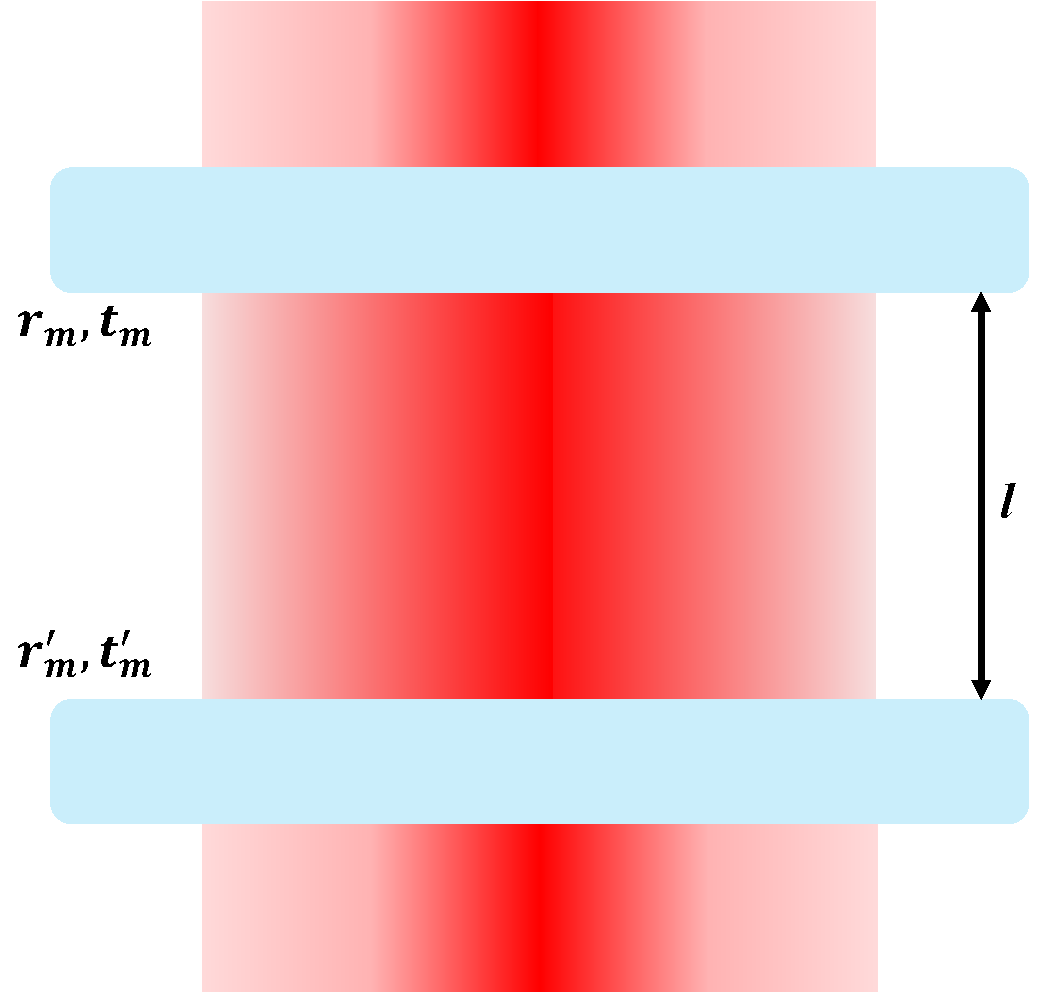
\includegraphics[width=\textwidth]{figures/broadband_sketch.pdf}
        \caption{Broadband cavity.}
    \end{subfigure}
    \hfill
    \begin{subfigure}[b]{0.3\textwidth}
        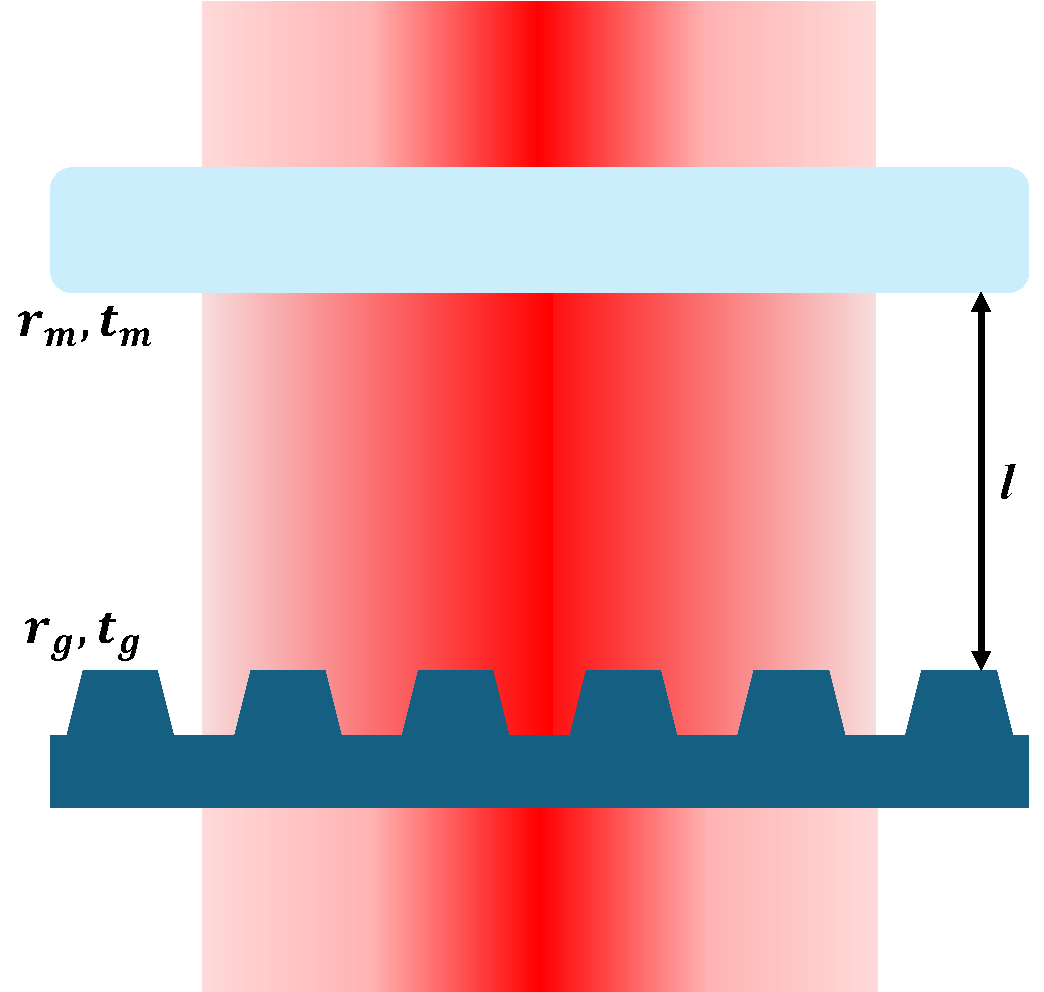
\includegraphics[width=\textwidth]{figures/single_fano_sketch.pdf}
        \caption{Single Fano cavity.}
    \end{subfigure}
    \hfill
    \begin{subfigure}[b]{0.3\textwidth}
        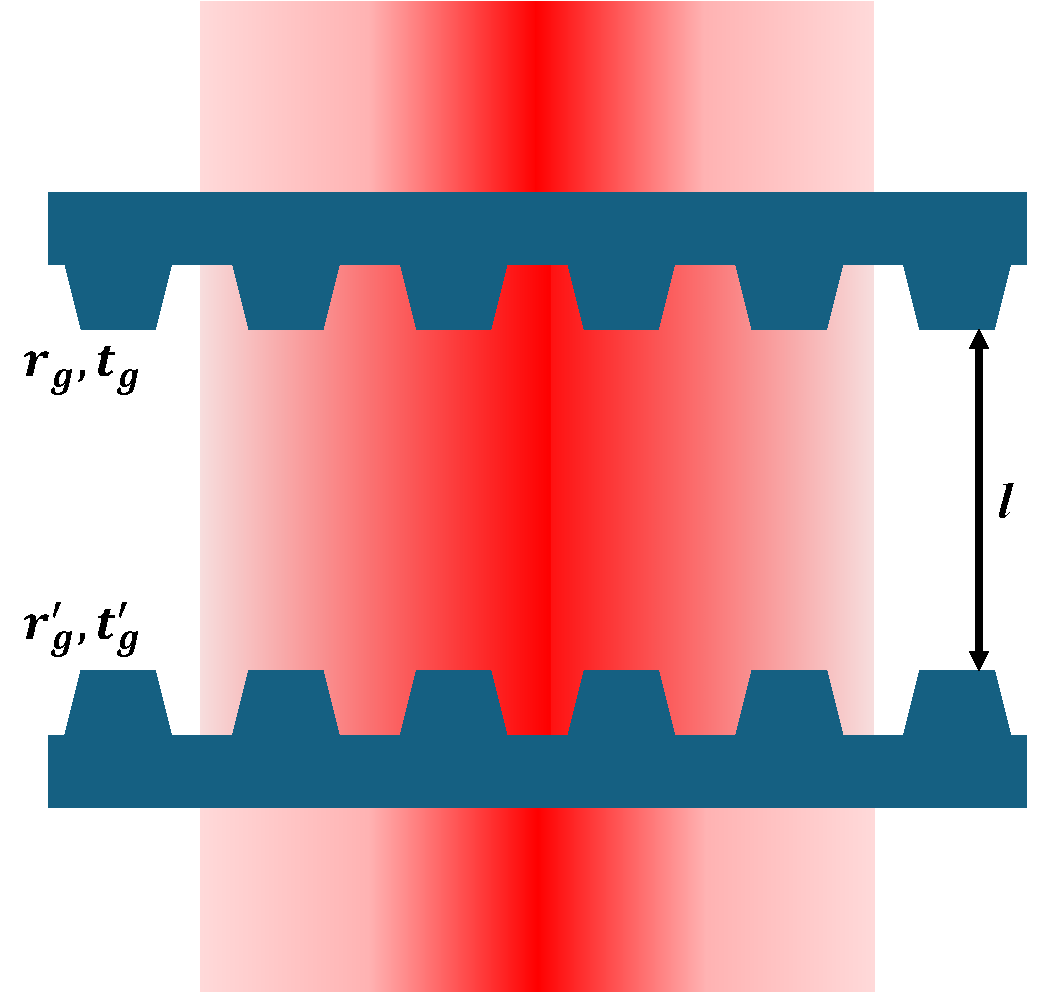
\includegraphics[width=\textwidth]{figures/double_fano_sketch.pdf}
        \caption{Double Fano cavity.}
    \end{subfigure}
\end{figure}


In this thesis I will present the theory of the sub-wavelength grating, i.e. Fano mirrors, and of the single- and double Fano cavities. I will show extensive simulations run for the transmission spectra of the double Fano cavity as a part of my investigation in order to map the on- and off-resonance behaviour as functions of various parameters. I will expand in detail on the experimental methods and techniques used in order to realize said theory and outline obstacles faced in that process. Finally I will present the results of my project and compare these with analytical predictions and discuss shortcomings and sources of error and noise of the setup and methods used. I will end by briefly dicussing the possible outlook of future projects regarding the double Fano cavity and the field of cavity electrodynamics generally in the light of my findings. 